%%!TEX TS-program = pdflatexmk
%%!TEX encoding = UTF-8 Unicode
\documentclass[11pt,french]{article}
\usepackage[utf8]{inputenc}

%\usepackage[letterpaper,body={6.0in,9.5in},vmarginratio=1:1]{geometry}
\usepackage[a4paper,twoside,textheight=24.6cm,heightrounded]{geometry}
\usepackage[small,compact]{titlesec}

%\usepackage{fourier}
%\usepackage[scaled=0.85]{berasans}
%\usepackage[scaled=0.85]{beramono}
%\usepackage{microtype}


\usepackage{xcolor}
%\usepackage[colorlinks, urlcolor=darkgray, linkcolor=darkgray]{hyperref}

\usepackage{graphicx}

\newcommand{\optkey}{\textsf{Opt}}
\newcommand{\ctlkey}{\textsf{Ctl}}
\newcommand{\cmdkey}{\textsf{Cmd}}
\newcommand{\esckey}{\textsf{Esc}}
\newcommand{\tabkey}{\textsf{Tab}}
\newcommand{\shiftkey}{\textsf{Shift}}

\newcommand{\mnu}[1]{\textsf{#1}}
\newcommand{\cmd}[1]{\textsf{#1}}
\newcommand{\To}{\,\(\to\)\,}

\pagestyle{plain}

\usepackage{varioref}
\usepackage{booktabs}

%\pagestyle{empty}

% set | as a command character within verbatim so you can execute commands there
\usepackage{verbatim}
\makeatletter
\addto@hook\every@verbatim{\catcode`|=0}
\makeatother

% define colored items to be inserted in verbatim environments
\usepackage{xcolor}
\setlength{\fboxsep}{0pt}
\newcommand{\selmark}{\colorbox{green}{\rule[-0.5ex]{0ex}{2.1ex}\texttt{•}}}
\newcommand{\selcom}{\colorbox{green}{\rule[-0.5ex]{0ex}{2.1ex}\texttt{•‹comment›}}}
\newcommand{\selcombwra}{\colorbox{green}{\rule[-0.5ex]{0ex}{2.1ex}\texttt{•‹placement: r,R,l,L,i,I,o,O›}}}
\newcommand{\selcomrule}{\colorbox{green}{\rule[-0.5ex]{0ex}{2.1ex}\texttt{•‹lift›}}}

% define a few items for easy use
\newcommand{\fastex}{Fas\hspace{-.15em}\TeX}
\newcommand{\TS}{\textsf{\TeX Shop}}
\newcommand{\TSVersion}{2.30}
\newcommand{\CCT}{\textsf{CommandCompletion.txt}}

%Polices : Fourier for math | Utopia (scaled) for rm | Helvetica for ss | Latin Modern for tt
\usepackage[upright]{fourier} % math & rm
\usepackage[scaled=0.85]{berasans}
\usepackage[scaled=0.85]{beramono}
%\usepackage[scaled=0.875]{helvet} % ss
%\renewcommand{\ttdefault}{lmtt} %tt\usepackage{scrtime}

%Babel
\usepackage{babel}
\addto\captionsfrench{\def\tablename{\scshape Tableau}}
\frenchbsetup{ShowOptions,og=«,fg=»}
\usepackage{xfrac}
\usepackage[decimalsymbol=comma,unitsep=cdot,digitsep=thick,mode=text,sepfour=true,valuesep=thick]{siunitx}
\usepackage[np,autolanguage]{numprint}

%Caption, float, microtype
\usepackage{caption}
\usepackage{float}
\usepackage[final,babel]{microtype}

%HYPERREF
\usepackage[colorlinks=true,linkcolor=black,urlcolor=blue]{hyperref}

\title{Complètement de commande avec \\ \TS\thanks{Traduit par René Fritz le 26 avril 2011.}}
%\title{Using Command Completion with \\ \TS}
\author{Herbert Schulz\\\small\href{mailto:herbs2@mac.com}{herbs2@mac.com}}
\date{2011/04/19}


\begin{document}
\maketitle
\thispagestyle{empty}

\section*{Introduction}

Depuis la version 1.34, \TS\ offrait un service de complètement de commande \emph{(Command Completion 
facility)} qui était assez puissante, bien que sous-utilisé. Le complètement de commande de \TS\ permet les achèvements (complètements) ou les substitutions (abréviations) pour un ensemble de caractères, délimités à gauche par un caractère de début de mot \emph{(Word Boundary Character)}\footnote{Ces caractères sont l'espace, la tabulation, le retour à la ligne (saut de ligne), le point, la virgule, le point-virgule, le deux-points, \{, \}, (, ) ou \textbackslash{} (en réalité le \textsf{\emph{TeX Command Character}} qui peut varier dans différentes implémentations). Le \{{} et \textbackslash{} font aussi partie de l'expansion.} et déclenchés par la touche d'échappement (\esckey).

%As of v1.34 \TS\ offered a Command Completion facility that was reasonably powerful, if under-utilized. Command Completion in \TS\ allows continuations (completions) or substitutions (abbreviations) for a set of characters bounded on the left by a \textsf{Word Boundary Character}\footnote{The \textsf{Word Boundary Characters} are space, tab, linefeed(newline), period, comma, semicolon, colon, \{, \}, (, ) or \textbackslash\ (actually the \textsf{TeX Command Character} which can vary in different implementations). The \{ and \textbackslash\ also become part of the expansion.} and triggered by the Escape (\esckey) key.

Avec l'aide des contributeurs de la liste mél de \textsf{Mac OS X TeX}\footnote{Souscrite en envoyant un mél à <\url{mailto:MacOSX-TeX-on@email.esm.psu.edu}>.}, un fichier \CCT\ a été créé en même temps que des macros Applescript associées pour tirer profit de ce service. Les complètements et abréviations fournis contiennent souvent des gros points « \texttt{•} » appelés repères \emph{(Marks)}\footnote{Précédemment appelés \emph{Tabs}.}, utilisés comme espaces réservés aux arguments de commande ou pour accéder facilement à la fin d'un environnement. Le saut à ces repères, vers l'avant ou vers l'arrière, a été obtenu en utilisant des macros\footnote{Le fichier original \CCT, les macros et la documentation sont encore disponibles sous le titre \textsf{CommandCompletion.zip} sur le site <\url{http://public.me.com/herbs2/}>.} ; les macros sautent aux 
repères, les sélectionnent ou les suppriment. La plupart des abréviations sont inspirées de celles employées dans le système \textsf{\fastex}\footnote{\textsf{\fastex} a été développé par Filip G. Machi, Jerrold E. Marsden et Wendy G. McKay. Pour de plus amples renseignements, consultez la page Web \textsf{\fastex}, <\url{http://www.cds.caltech.edu/~fastex/}>.} utilisé avec \textsf{TypeIt4Me}\footnote{\textsf{TypeIt4Me}, par Riccardo Ettore, qui 
est actuellement un panneau de préférences, permet de remplacer une abréviation dans la plupart des programmes 
OS~X avec « des dictionnaires » qui peuvent dépendre d'une application. Voir la page web \textsf{TypeIt4Me}, <
\url{http://www.typeit4me.com/}, pour plus d'informations.}.
%\enlargethispage*{1.5\baselineskip}

%With the help of the good folks on the \textsf{Mac OS X TeX} e-mail list\footnote{Subscribe by sending an e-mail to <\url{mailto:MacOSX-TeX-on@email.esm.psu.edu}>.}, a \CCT\ file was created along with associated Applescript macros to take advantage of that facility. The completions and abbreviations supplied often contain bullet characters, `\texttt{•}', called Marks\footnote{Previously called Tabs.}, as placeholders for command arguments or to easily get to the end of an environment. Skipping forward and backward to these Marks was accomplished using macros\footnote{The original \CCT\ file, macros and documentation are still available as \textsf{CommandCompletion.zip} from  <\url{http://public.me.com/herbs2/}>.}; the macros jumped to the Marks and selected, or deleted, them. Most of the abbreviations were inspired by those used in the \textsf{\fastex}\footnote{\textsf{\fastex} was developed by Filip G. Machi, Jerrold E. Marsden and Wendy G. McKay. For more information see the \textsf{\fastex} web page, <\url{http://www.cds.caltech.edu/~fastex/}>.} set used with \textsf{TypeIt4Me}\footnote{\textsf{TypeIt4Me}, by Riccardo Ettore, presently a preference pane, allows abbreviation replacement in most OS~X programs with ``dictionaries'' that can be application dependent. See the \textsf{TypeIt4Me} web page, <\url{http://www.typeit4me.com/}>, for more information.}.

À partir de la version 2.30, \TS\ intègre une version améliorée du complètement de commande inspirée 
de Hugh Neary et Will Robertson. Les macros Applescript ne sont plus nécessaires et les arguments des 
complètements peuvent comporter un bref aide-mémoire.

%Version 2.30 and later of \TS\ offers a built-in and enhanced version of Command Completion inspired by Hugh Neary and Will Robertson. There is no longer a need for the Applescript macros and the arguments of completions can have short comments.

{\bfseries\TS\ 2.36 permet de déclencher le complètement de commande par la touche Tab (\tabkey) et de revenir à la touche \esckey\ en allant dans : \mnu{TeXShop}\To\mnu{Préférences…}\To\ \mnu{Document}\To\mnu{Commande de complétion déclenchée par}. Partout où vous verrez dans ce document \esckey\ utilisez \tabkey\ si vous avez opté pour ce nouveau réglage.}

%{\bfseries\TS\ 2.36 introduced the ability to switch the Command Completion trigger key between Tab (\tabkey) and the \esckey\ keys in \mnu{TeXShop}\To\mnu{Preferences}\To\mnu{Source}\To\mnu{Command Completion Triggered By:}. Wherever you see \esckey\ in this document use \tabkey\ if you've set that as the trigger.}

{\bfseries À partir de \TS\ 2.38, le complètement de commande maintient le retrait de ligne.} Dans \path{~/Library/TeXShop/CommandCompletion/IndentedCC/}, on trouve également une version du fichier \CCT\ avec retrait de ligne. Elle peut être activée en la copiant dans \path{~/Library/TeXShop/CommandCompletion/} afin de remplacer la version qui s'y trouve. Pour obtenir la version originale du fichier \CCT{}, il suffit de déplacer le dossier \path{~/ Library/TeXShop/CommandCompletion/} sur votre bureau et de redémarrer \TS.


%{\bfseries Command Completion in \TS\ 2.38 and later preserves indentation.} Also included is an indented version of the \CCT\ file. It is found in \path{~/Library/TeXShop/CommandCompletion/IndentedCC/} and is activated by copying the file located there into \path{~/Library/TeXShop/CommandCompletion/} thus overwriting the version already there. To get the original version of the \CCT\ file back simply move the \path{~/Library/TeXShop/CommandCompletion/} folder to your Desktop and restart \TS.

\section*{Installation}

Placer simplement cette version de \TS\ dans \path{/Applications/TeX/}. Si vous avez déjà utilisé une précédente 
version de \TS\ (antérieure à \TSVersion) suivez également les instructions de la sous-section suivante.

%Simply place this version of \TS\ into \path{/Applications/TeX/}. If you ever started up an older version of \TS\ (earlier than \TSVersion) also follow the directions in the following sub-section.

\subsection*{\CCT}

Une nouvelle version, par défaut, de \CCT\ est incorporée dans cette nouvelle version de \TS. Elle sera installée, avec les autres fichiers, à la première exécution de \TS{}, \emph{sauf} si vous aviez utilisé \TS\ auparavant. Dans ce cas, vous devez déplacer le répertoire \path{~/Library/TeXShop/CommandCompletion/} (\path{~} est votre répertoire personnel) sur votre bureau et démarrer la nouvelle version de \TS{}; un dossier de remplacement avec la nouvelle version de \CCT\ sera créé.

%A new default version of \CCT\ is embedded within this new version of \TS. It will get installed, along with other files, the first time \TS\ runs \emph{unless} you've used \TS\ before. In that case you need to move the \path{~/Library/TeXShop/CommandCompletion/} (\path{~} is your HOME directory) directory to your Desktop and start the new version of \TS; a replacement folder with the new version of \CCT\ will be created.

Si vous avez déjà ajouté des éléments au dossier original, vous serez en mesure de les fusionner dans le nouveau 
fichier après sa création. Vous pouvez ouvrir la nouvelle version de \CCT\ en cliquant sur l'élément final du menu \mnu{Source}\To\mnu{Commande de complètement}\To\ \mnu{Éditer le fichier de la commande…}. L'ancien fichier doit être ouvert avec le codage Unicode (UTF-8) : utilisez la commande du menu \mnu{Fichier}\To\mnu{Ouvrir…} (\cmd{\cmdkey-O}) et assurez-vous d'avoir sélectionné le codage \texttt{Unicode(UTF-8)} avant d'ouvrir votre ancienne version dans \TS.

%If you've already added items to the original file you will be able to merge them into the new file after it's created. You can open the new version of \CCT\ by clicking on the \mnu{Source}\To\mnu{Command Completion}\To\mnu{Edit Command Completion File\dots} menu item. The older file \emph{must} be opened with Unicode (UTF-8) encoding: use the \mnu{File}\To\mnu{Open\dots} (\cmd{\cmdkey-O}) menu command and make sure to select the \textsf{Unicode (UTF-8)} encoding before opening your old version in \TS.

\section*{Nouveautés dans \TS}
%\section*{Some of What's New in \TS}

Quatre changements interconnectés à \TS{} sont des plus importants : un ajout à la façon dont \TS{} traite 
les complètements à partir du fichier \CCT\ ; un nouveau menu qui a des commandes pour 
rechercher et sélectionner les repères (\emph{Marks}) dans les complètements ; la possibilité de joindre des aide-mémoire aux repères ; un nouveau fichier \CCT\ qui acquiert un certain avantage 
des trois précédents changements. Les quatre sous-sections suivantes traitent de chacun de ces changements plus 
en détail. Quelques changements mineures, au niveau du menu, sont examinés séparément.

%Most important are four interconnected changes to \TS: an addition to the way \TS\ handles completions from \CCT; a new menu that has commands for searching and selecting Marks within completions; the ability to have comments attached to Marks; a new \CCT\ file that takes some advantage of the previous three changes. The following four sub-sections cover each of these changes in more detail. Some minor menu changes are discussed separately.

\subsection*{Traitement du complètement}
%\subsection*{Changes to Completion Handling}

Les complètements (dans le fichier \CCT) dans les versions précédentes de \TS{} ne 
pouvaient contenir qu'une seule commande \texttt{\#INS\#} pour positionner le point d'insertion en leur sein. 

Cette version \TS{} permet aux complètements d'avoir \emph{deux} copies de \texttt{\#INS\#} entre lesquelles le texte sera sélectionné. Un seul \texttt{\#INS\#} se comporte de la même façon qu'auparavant ; il y a une totale compatibilité ascendante avec les versions précédentes de \TS.

%Completions (in the \CCT\ file) in previous versions of \TS\ could contain a single \verb|#INS#| command for the positioning of the insertion point within the completion.
%
%This version of \TS\ allows completions to have \emph{two} copies of \verb|#INS#| and the text between them is selected. A single \verb|#INS#| behaves the same as before; there is complete backward compatibility with the previous versions of \TS.

\subsection*{Nouveau menu \mnu{Source}\To\mnu{Commande de complètement}\To\mnu{Repères}}
%\subsection*{The \mnu{Source}\To\mnu{Command Completion}\To\mnu{Marks} Menu}

%The new \mnu{Source}\To\mnu{Command Completion}\To\mnu{Marks} menu contains commands to search for, move to and select Marks and Comments. The commands are shown in Table (\ref{tbl:menu}) on page \pageref{tbl:menu}.

Le nouveau menu \mnu{Source}\To\mnu{Commande de complètement}\To\mnu{Repères} contient des commandes pour 
rechercher, aller au niveau et sélectionner les repères et les aide-mémoire. Les commandes figurent 
dans le \textsc{Tableau}~\Vref{tbl:menu}.
\begin{table}[htbp]
\centering
\caption{Commandes du menu \mnu{Source}\To\mnu{Commande de complètement}\To\mnu{Repères}.\label{tbl:menu}}
\begin{tabular}{l l p{6.6cm}}
{\bfseries Éléments du menu} & {\bfseries Raccourci} & {\bfseries Connexion interne} \\
\cmidrule[0.5pt](lr){1-1} \cmidrule[0.5pt](lr){2-2} \cmidrule[0.5pt](lr){3-3}
\sffamily Repère suivant &  \ctlkey\,-\,\cmdkey\,-\,\textsf{F} & Va au prochain repère \emph{(Mark)} ou aide-mémoire. \\
\sffamily Repère suivant (Ôter) & \ctlkey\,-\,\optkey\,-\,\cmdkey\,-\,\textsf{F} & Va au prochain repère ou aide-mémoire, le sélectionne et supprime le repère : c'est surtout utile, quand vous avez des environnements imbriqués, pour supprimer automatiquement un repère situé à la fin d'un environnement interne.\\
\sffamily Repère précédent & \ctlkey\,-\,\cmdkey\,-\,\textsf{G} & Inverse de \textsf{Repère suivant}. \\
\sffamily Repère précédent (Ôter) & \ctlkey\,-\,\optkey\,-\,\cmdkey\,-\,\textsf{G} & Inverse de \textsf{Repère suivant (Ôter)}.  \\
\sffamily Insérer un repère & \cmdkey\,-\,\textsf{8} & Place un repère au point d'insertion. Utilisé pour repérer des arguments, etc., lors de la création de nouveaux complètements dans le fichier \CCT. \\
\sffamily Insérer un aide-mémoire & \ctlkey\,-\,\cmdkey\,-\,\textsf{8} & Place l'ossature d'un aide-mémoire, « •‹› » avec le point d'insertion situé avant « › » : pratique pour créer des commentaires dans le fichier \CCT. \\
\end{tabular}
\end{table}
Les versions \mnu{(Ôter)} des commandes de recherche ne sont visibles dans le menu que si la touche Option (\optkey) est appuyée et la commande \mnu{Insérer un aide-mémoire} ne s'affiche que lorsque vous maintenez appuyée la touche Contrôle (\ctlkey). La commande \mnu{Insérer un repère} est ajoutée grâce à la fonction de raccourci clavier de \TS{} (précédemment appelé auto-complètement \emph{(Auto Complete)}) qui va inserrer un \texttt{\textbackslash bullet} dans le document lorsque la combinaison de touches qui, normalement, insère un « • » (\mnu{\optkey-8} dans la correspondance du clavier américain) est employée. La version par défaut du menu \mnu{Repères} est montrée dans la \textsc{Figure}~\Vref{fig:marks}.  
%\begin{table}
%\centering
%\begin{tabular}{llp{6.7cm}}
%{\bfseries Menu Item} & {\bfseries Shortcut} & {\bfseries Internal Connection} \\
%\cmidrule[0.5pt](lr){1-1} \cmidrule[0.5pt](lr){2-2} \cmidrule[0.5pt](lr){3-3}
%\sffamily Next Mark & \ctlkey\,-\,\cmdkey\,-\,\textsf{F} & Jump to and select the next Mark and/or Comment. \\
%\sffamily Next Mark (Del) & \ctlkey\,-\,\optkey\,-\,\cmdkey\,-\,\textsf{F} & Jump to and select the next Mark and/or Comment and delete the Mark. This is most useful when you have nested environments to automatically delete a Mark at the end of an inner environment.  \\
%\sffamily Previous Mark & \ctlkey\,-\,\cmdkey\,-\,\textsf{G} & Like \textsf{Next Mark} but search backwards. \\
%\sffamily Previous Mark (Del) & \ctlkey\,-\,\optkey\,-\,\cmdkey\,-\,\textsf{G} & Like \textsf{Next Mark (Del)} but search backwards. \\
%\sffamily Insert Mark & \cmdkey\,-\,\textsf{8} & Places a Mark at the insertion point. Used to mark arguments, etc., when creating new completions in \CCT. \\
%\sffamily Insert Comment & \ctlkey\,-\,\cmdkey\,-\,\textsf{8} & Places a Comment Skeleton, ``•‹›'' with the insertion point before the ``›'', at the insertion point. Handy for creating comments in \CCT. \\
%\end{tabular}
%\caption{Commands in the \mnu{Source}\To\mnu{Command Completion}\To\mnu{Marks} Menu.\label{tbl:menu}}
%%\label{tbl:menu}
%\end{table}
%The \mnu{(Del)} versions of the search commands only show in the menu when the Option (\optkey) key is pressed and the \texttt{Insert Comment} command only appears when you hold down the Control (\ctlkey) key. The \mnu{Insert Mark} command is added since using \TS's Key Binding (previously called Auto Complete) facility will insert \texttt{\textbackslash bullet} in the document when the keystroke that normally inserts a `•' (\mnu{\optkey-8} with a \textsc{US} keyboard mapping) is pressed. The default version of the \mnu{Marks} menu is shown in Figure (\ref{fig:marks}) on page \pageref{fig:marks}.

\begin{figure}[htbp]
\centering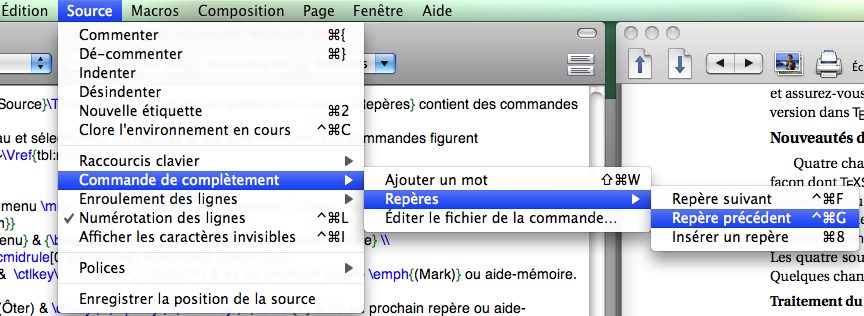
\includegraphics[width=\textwidth]{figs/mark}
\caption{Menu, par defaut, de \mnu{Source}\To\mnu{Commande de complètement}\To\mnu{Repères}.\label{fig:marks}}
%\caption{The Default \mnu{Source}\To\mnu{Command Completion}\To\mnu{Marks} Menu.}
\end{figure}

\subsection*{Aide-mémoire}
%\subsection*{Comments}

Les modifications mentionnées dans les sous-sections précédentes permettent aux complètements de contenir des 
aide-mémoire -- petits « pense-bêtes » -- qui donnent des indications sur ce que doit contenir un argument donné. 
Les aide-mémoire, entourés de « •‹ » et « › »\footnote{Notez que « \texttt{‹} » et « \texttt{›} » sont des guillemets simples et non les glyphes « < » et « > ».}, sont placés à l'intérieur des arguments ; si le premier argument contient un aide-mémoire, celui-ci doit être entouré de deux \verb|\#INS\#| afin qu'il soit sélectionné d'abord.

%The changes mentioned in the previous sub-sections allow completions to contain Comments---short ``memory joggers'' that have some information about the contents of a given argument. The comments are contained within arguments and are surrounded by ``•‹'' and ``›\footnote{Note that `\texttt{‹}' and `\texttt{›}' are single ``guillemot'' glyphs, not `<' and `>'.}'' within the arguments; if the first argument contains a comment it should be surrounded by two \verb|#INS#| so it is the initial selection.

\subsection*{Nouveau fichier \CCT}
%\subsection*{The New \CCT\ File}

Par rapport à la version originale, il y a quelques changements dans le nouveau fichier \CCT\ qui vient avec cette version de \TS\ :
\begin{itemize}
\item Il y a quelques corrections, mineures, de bogues, et quelques environnements et commandes supplémentaires ;
\item toutes les commandes \verb|#INS#| isolées sont remplacées par des \verb|#INS#•#INS#| afin que 
le repère initial soit sélectionné, \selmark. Il s'agit d'un souci de cohérence entre l'apparence et le comportement 
lorsque vous utilisez les commandes \mnu{Repère suivant/précédent} ;
\item il y a un peu (trop peu?) d'exemples d'aide-mémoire dans les commandes et les environnements.
\end{itemize}

%There are a few changes to the new \CCT\ file that comes with this version of \TS\ when compared to the one supplied with the original add-on version:
%\begin{itemize}
%\item
%there are some minor bug fixes and a few additional environments and commands;
%\item
%all single \verb|#INS#| commands are replaced by \verb|#INS#•#INS#| so that the initial selection is a selected Mark, \selmark. This is for consistency with the appearance and behavior when using the \texttt{Next/Previous Mark} commands;
%\item
%there are a few (too few?) examples of comments in commands and environments.
%\end{itemize}

\subsection*{Nouveaux raccourcis clavier dans \TS{} à partir de 2.36}
%\subsection*{Additional Shortcuts in \TS\ 2.36 and Later}

En plus de \ctlkey\,-\,\cmdkey\,-\,\textsf{F/G} pour, \mnu{Repère suivant} et \mnu{Repère précédent}, \TS{} 2.36 introduit le raccourci \optkey/\ctlkey\,-\,\esckey\ comme alternative pour atteindre ces éléments de menu. Si vous voulez supprimer cette disposition, éxécutez la commande suivante :
\begin{verbatim}
defaults write TeXShop CommandCompletionAlternateMarkShortcut NO
\end{verbatim}
dans le \texttt{Terminal}. Pour revenir au réglage précédent remplacer \texttt{NO} par \texttt{YES}.  

%Besides \ctlkey\,-\,\cmdkey\,-\,\texttt{F/G} for \mnu{Next/Previous Mark} \TS\ 2.36 introduced the \optkey/\ctlkey\,-\,\esckey\ as alternates for those menu items. If you wish to turn that feature off execute the command
%\begin{verbatim}
%defaults write TeXShop CommandCompletionAlternateMarkShortcut NO
%\end{verbatim}
%in \texttt{Terminal} to turn it off or substitute \texttt{YES} for \texttt{NO} in the command to turn it back on.

\section*{Utilisation}
%\section*{Usage}

\subsection*{Complètement de commande}
%\subsection*{Command Completion}

Une utilisation typique du complètement de commande est d'installer des environnements. Pour ce faire, tapez 
\verb|\b| puis \esckey ; ce qui devrait vous donner \verb|\begin{|. Ensuite, commencez à taper le nom de l'environnement, p. ex., \verb|eq| puis \esckey\ ce qui donnera : 
\begin{verbatim}
\begin{equation}
|selmark
\end{equation}•
\end{verbatim}
tandis que l'\esckey\ suivant donnera \texttt{eqnarray} suivi de sa variante étoilée (\texttt{*}). Après avoir entré le 
texte de votre équation au niveau du curseur exécutez la commande \mnu{Source}\To\ \mnu{Commande de complètement}\To\ \mnu{Repères}\To\mnu{Repère suivant} et le curseur sélectionnera (ou supprimera, si \mnu{Repère suivant 
(Ôter)} est utilisé) le « \texttt{•} » suivant et vous pourrez commencer à taper le texte qui suit.

Les macros sont également très pratiques pour les commandes qui prennent plusieurs arguments. Par exemple, 
pour créer une nouvelle commande avec un argument optionnel tapez \verb|\new| ou \verb|\newc| puis trois fois \esckey\ pour obtenir : 
\begin{verbatim}
\newcommand{|selmark}[•][•]{•}
\end{verbatim}
avec le premier repère sélectionné. Après avoir entré le nom de la nouvelle commande utilisez la 
commande \mnu{Repère suivant} pour passer à l'argument suivant, etc.

%A typical use of command completion is to set up environments. To do this type \verb|\b| and \esckey; this should get you \verb|\begin{|. Then start to type the environment name; e.g., \verb|eq| and \esckey\ will give
%\begin{verbatim}
%\begin{equation}
%|selmark
%\end{equation}•
%\end{verbatim}
%while the next \esckey\ gives \texttt{eqnarray} followed by it's \texttt{*}-variant. After entering your equation text at the cursor run the \mnu{Source}\To\mnu{Completion}\To\mnu{Marks}\To\mnu{Next Mark} command and the cursor will select (and  delete if \mnu{Next Mark (Del)} is used) the next `\texttt{•}' so you can start to type following text.
%
%The macros are also handy for commands that take multiple arguments. For example, to create a new command with an optional argument type \verb|\new| or \verb|\newc| and then \esckey\ three times to get
%\begin{verbatim}
%\newcommand{|selmark}[•][•]{•}
%\end{verbatim}
%with the first mark selected. After entering the new command's name use the \texttt{Next Mark} command to jump to the next argument, etc.

\subsection*{Abréviations}
%\subsection*{Abbreviations}

En plus du complètement de commande, il existe aussi de nombreuses abréviations pour les commandes. La 
principale différence est que les abréviations ne sont pas seulement le début d'un nom de commande. Par exemple, 
taper \texttt{benu}, puis \esckey\ \emph{au début d'une ligne}\footnote{Ou après tout autre caractère de début de mot \emph{(\texttt{Word Boundary Character})}.} produira l'environnement complet d'une énumération :
\begin{verbatim}
\begin{enumerate}
\item
|selmark
\end{enumerate}•
\end{verbatim}
comme vous pouvez vous en douter. De telles abréviations existent pour de nombreux environnements, ainsi que pour des commandes de sectionnement. D'autres versions de commande avec une ou plusieurs options ou des variantes étoilées (\texttt{*}) ont des noms qui se terminent respectivement par « \texttt{o} » (un ou plusieurs) ou « \texttt{s} » : p. ex., \texttt{sec} et deux pressions sur \esckey\ ou \texttt{secs} et une seule pression sur \esckey\ au début d'une nouvelle ligne donnent \verb|\section*{|\selmark\verb|}|. Par ailleurs, après avoir tapé le texte pour le premier item, taper \texttt{it} puis \esckey\ sur une nouvelle ligne va produire un autre \verb|\item| avec un repère sélectionné sur la ligne du dessous ; des pressions successives sur la touche \esckey\ donneront \verb|\item[|\selmark\verb|]| avec un repére sur la ligne suivante, \verb|\textit{|\selmark\verb|}| et enfin \verb|\itshape| avant de retourner au \texttt{it} d'origine.

%In addition to command completion there also exist many abbreviations for commands. The principal difference is that the abbreviations are not just the start of a command name. For example typing \texttt{benu} and then \esckey\ \emph{at the beginning of a line}\footnote{Or after any other \texttt{Word Boundary Character}.} will produce the complete enumerated list environment:
%\begin{verbatim}
%\begin{enumerate}
%\item
%|selmark
%\end{enumerate}•
%\end{verbatim}
%as you might expect. Abbreviations like this exist for many environments as well as sectioning commands. Alternate command versions with one or more options or \texttt{*}-variants have names that end with `\texttt{o}' (one or more) or `\texttt{s}' respectively: e.g., \texttt{sec} and two presses of \esckey\ or \texttt{secs} and a single \esckey\ at the start of a new line give \verb|\section*{|\selmark\verb|}|. By the way, After typing the text for the first item, typing \texttt{it} and \esckey\ on a new line will generate another \verb|\item| with a selected Mark on the line below it; continued presses of \esckey\ will give \verb|\item[|\selmark\verb|]| with a Mark on the following line, \verb|\textit{|\selmark\verb|}| and finally \verb|\itshape| before returning to the original \texttt{it}.

Vous devez vous souvenir qu'il faut un des caractères de début de mot, avant d'utiliser les abréviations ; sinon, la 
substitution ne fonctionnera pas correctement. Ce n'est pas un problème avec les environnements et les commandes 
de sectionnement, puisque vous commencez, généralement, sur une nouvelle ligne ; mais, cela peut l'être pour 
d'autres abréviations. C'est pourquoi de nombreuses abréviations ont également une version avec « \verb|\| » ; p. 
ex., \texttt{\`{}tt} puis \esckey\ ne se développera pas correctement, puisque « \texttt{\`{}} » n'est pas un caractère de 
début de mot tandis que \texttt{\`{}\textbackslash tt} puis \esckey\ donnera \texttt{\`{}\textbackslash texttt\{\selmark\}} et qu'une deuxième pression de la touche \esckey\ donnera la déclaration \texttt{\`{}\textbackslash ttfamily}\footnote{Des abréviations similaires existent pour les \texttt{bf}, \texttt{sf}, \texttt{sc}, etc. Les versions pour les maths sont précédées par un \texttt{m}, par exemple, \texttt{mbf} puis \esckey\, donnera \texttt{\textbackslash mathbf\{\selmark\}}.}


%You must remember to have one of the \textsf{Word Boundary Characters} before use or the substitution won't operate properly. This a not a problem with environments and sectioning commands, since you usually start them on a new line, but can be for other abbreviations. Therefore many abbreviation also have a `\verb|\|' version; e.g., \texttt{\`{}tt} and \esckey\ will not expand properly since the `\texttt{\`{}}' isn't a \textsf{Word Boundary Character} while \texttt{\`{}\textbackslash tt} and \esckey\ will expand to \texttt{\`{}\textbackslash texttt\{\selmark\}} while a second \esckey\ will give the declaration \texttt{\`{}\textbackslash ttfamily}\footnote{Similar abbreviations exist for \texttt{bf}, \texttt{sf}, \texttt{sc}, etc. Math versions have a preceding \texttt{m}; e.g., \texttt{mbf} and \esckey\ will give \texttt{\textbackslash mathbf\{\selmark\}}.}.

Bon nombre des caractères grecs et leurs versions mathématiques, en ligne, ont des abréviations dont les règles 
sont les suivantes :
\begin{enumerate}
\item Les abréviations des caractères grecs commencent toutes par un « \texttt{x} » suivi d'une notation pour les 
caractères : p. ex., \verb|xa| ou \verb|\xa|\footnote{Toutes les abréviations des caractères grecs ont une 
version \texttt{\textbackslash}.} puis \esckey\ donnera \verb|\alpha|.
\item La version \texttt{var} de plusieurs caractères grecs commencent par « \texttt{xv} » suivi de la notation 
pour le caractère : p. ex., \texttt{xth} donne \verb|\theta| tandis que \verb|xvth| puis \esckey\ donne \verb|\vartheta|.
\item Pour obtenir des lettres capitales utilisez un « \texttt{xc} » : p. ex., \verb|xg| donne \verb|\gamma| tandis que \verb|xcg| donne \verb|\Gamma|.
\item Enfin, l'abréviation précédée d'un « \texttt{d} » présente le caractère grec comme dans une équation 
mathématique en ligne : p. ex., \verb|dxcd| donne \verb|\(\Delta\)|.
\end{enumerate}

%Many of the Greek characters and in-line math versions of the Greek characters have abbreviations with the following rules:
%\begin{enumerate}
%\item
%The abbreviations for Greek characters all start with an `\texttt{x}' and a notation for the character: e.g., \verb|xa| or \verb|\xa|\footnote{All of the Greek character abbreviations have \texttt{\textbackslash} versions.} and \esckey\ give \verb|\alpha|. 
%\item
%The \texttt{var} version of several Greek characters start with `\texttt{xv}' and the notation for the character: e.g., \texttt{xth} gives \verb|\theta| while \verb|xvth| and \esckey\ gives \verb|\vartheta|.
%\item
%To get capitals for some letters use an `\texttt{xc}': e.g., \verb|xg| gives \verb|\gamma| while \verb|xcg| gives \verb|\Gamma|.
%\item
%Finally, preceding by a `\texttt{d}' gives the following Greek character as an in-line math equation: e.g., \verb|dxcd| gives \verb|\(\Delta\)|.
%\end{enumerate}

Les abréviations seront complétées et bouclées par le biais des correspondances tout comme les complètements de 
commande : par exemple, l'abréviation \texttt{newcoo} (notez le « \texttt{oo} » à la fin de l'abréviation) suivi 
d'une pression sur \esckey\ ou \texttt{newc} suivi de trois pressions sur la touche \esckey{}, les deux placées sur une nouvelle ligne, donneront \verb|\newcommand{|\selmark\verb|}[•][•]{•}|, le \verb|\newcommand| avec deux arguments optionnels. Il existe des abréviations de remplacement pour certaines commandes : p. ex., \texttt{ncm} donne le même résultat que  \texttt{newc}. 

Je vous suggère de lire le fichier \CCT\ pour voir les abréviations disponibles ; toutes les lignes avec « \kern-1.7pt\texttt{:=} » sont des abréviations. Naturellement, vous pouvez les modifier selon vos besoins, en ajouter ou 
en supprimer.

%Abbreviations will be completed and cycle through matches just like the command completions: e.g., both the abbreviation \texttt{newcoo} (note the `\texttt{oo}' at the end of the abbreviation) and \esckey\ or \texttt{newc} followed by three \esckey\ key presses on a new line give \verb|\newcommand{|\selmark\verb|}[•][•]{•}|, the \verb|\newcommand| with two optional arguments. There are alternate abbreviations for some commands: e.g., \texttt{ncm} gives the same result as \texttt{newc}.
%
%I suggest that you read through the \CCT\ file to see what abbreviations are available; all lines with `\kern-1.7pt\texttt{:=}' are abbreviations. Naturally, you can change them to suit your needs and add and delete others.

\subsection*{Aide-mémoire}
%\subsection*{Comments}

Il est facile de se souvenir des arguments des commandes utilisées assez souvent, mais ce n'est pas le cas pour 
celles qui le sont rarement. Ces dernières sont toutes indiquées pour les aide-mémoire. L'ordre des arguments de la 
commande \verb|\rule| en est un exemple ; Tapez \verb|\rul| et deux fois \esckey\ pour obtenir \verb|\rule[|\selcomrule\verb|]{•‹width›}{•‹height›}|, la version avec l'argument optionnel\footnote{Soit, \texttt{\textbackslash rule[\#INS\#•‹lift›\#INS\#]\{•‹width›\}\{•‹height›\}} dans le fichier \CCT.}. Un autre exemple est l'environnement \texttt{wrapfigure} de l'extension \texttt{wrapfig}, qui dispose de versions différentes par le nombre et les positionnements des arguments facultatifs. Pour voir les variations avec les aide-mémoire, tapez \texttt{bwr} sur une ligne vide et appuyez sur \esckey\ pour obtenir :
\begin{verbatim}
\begin{wrapfigure}{|selcombwra}{•‹width›}
•
\end{wrapfigure}•
\end{verbatim}
pour les versions comportant des arguments optionnels appuyez successivement sur \esckey.


%It is easy to remember the arguments for commands that are used fairly often but to forget those rarely used; these are the perfect candidates for comments. E.g., the order of the arguments for the \verb|\rule| command; type \verb|\rul| and \esckey\ twice to get \verb|\rule[|\selcomrule\verb|]{•‹width›}{•‹height›}|, the version with the optional argument\footnote{This is \texttt{\textbackslash rule[\#INS\#•‹lift›\#INS\#]\{•‹width›\}\{•‹height›\}} in the \CCT\ file.}. Another example is the \texttt{wrapfigure} environment, from the \texttt{wrapfig} package, which has multiple versions with differing numbers and positions of optional arguments. To see the variations with the comments type \texttt{bwr} on an empty line and press \esckey\ to get:
%\begin{verbatim}
%\begin{wrapfigure}{|selcombwra}{•‹width›}
%•
%\end{wrapfigure}•
%\end{verbatim}
%with the versions with optional arguments on succeeding presses of \esckey.

\subsection*{Autres environnements}
%\subsection*{Other Environments}

Les environnements non prédéfinis dans le fichier \CCT\ peuvent, toujours, être ajoutés si vous les utilisez beaucoup, mais il y a une alternative pour une utilisation occasionnelle. Les environnements peuvent être construits à l'intérieur même de l'algorithme de complètement. Tapez d'abord \verb|\b| et appuyez sur \esckey\ pour obtenir \verb|\begin{|, entrez ensuite le nom d'environnement et l'accolade de fermeture \texttt{\}}, appuyez de nouveau sur \esckey\ et la commande de clôture \verb|\end{}| avec le nom correspondant de l'environnement sera produite sur une ligne distincte.

%Environments that aren't built into the \CCT\ file can always be added if you use them a lot but there is an alternative for occasional use. Built into the completion algorithm is a way to complete environments. First press \verb|\b| and \esckey\ to get \verb|\begin{|, enter the environment name and the closing \texttt{\}} and then \esckey\ again; the closing \verb|\end{}| with the corresponding environment name will be generated on a separate line.

\section*{Abréviations du fichier \CCT}
%\section*{Abbreviations in \CCT}

Cette section contient, nous l'espérons, la liste complète des abréviations fournies dans \CCT. La liste a été partagée entre, les environnements, les commandes et les déclarations, et les lettres grecques. Si vous donnez le début d'une abréviation la recherche va commencer par la première abréviation similaire à votre proposition et à chaque pression de \esckey\ elle va descendre dans la liste jusqu'à ce qu'il n'y ait plus aucune identité : p.~ex., si vous tapez \texttt{be} des pressions successives de \esckey\ correspondront à \texttt{benu}, \texttt{benuo}, \texttt{bequ}, \texttt{bequs}, \texttt{beqn} et \texttt{beqns} avant de retourner à l'original \texttt{be}. Ajouter plus de lettres à l'abréviation peut vous permettre d'arriver au résultat escompté en utilisant moins souvent la touche \esckey. En réalité, certaines des commandes et déclarations sont éparpillées entre les environnements dans le fichier \CCT\ si bien qu'il pourrait y avoir, parfois, des éléments en plus. Les tableaux ne présentent pas les complètements standards ni les versions « \verb"\" » des abréviations.%\smallskip

%This section contains a, hopefully, complete list of the abbreviations supplied in the latest \CCT. The list has been broken up into Environments, Commands \& Declarations and Greek Letters. If you supply a certain beginning abbreviation the search will start at the first match to what you supply and succeeding presses of \esckey\ will go down the list until there is no longer a match; e.g. if you type \texttt{be} succeeding presses of \esckey\ will match \texttt{benu}, \texttt{benuo}, \texttt{bequ}, \texttt{bequs}, \texttt{beqn} and \texttt{beqns} before returning to the original \texttt{be}. Adding more letters to the abbreviation may get you to the desired completion with fewer presses of \esckey. In reality some of the Commands \& Declarations are scattered between the Environments in the \CCT\ file so there might be additional items at times. The tables don't include standard completions or the `\verb"\"' versions of the abbreviations.

\noindent\textbf{\textsc{Remarque}. -- La liste peut sembler un peu intimidante. Il n'est pas nécessaire de « mémoriser » toutes ces abréviations ; apprenez-en un nombre minimum, celles dont vous avez besoin, et utilisez la touche \esckey{} pour obtenir les variations d'une abréviation donnée (voir \textsc{Figure}~\Vref{fig:sec}).}
\begin{figure}\centering
\makebox[\textwidth]{
\fbox{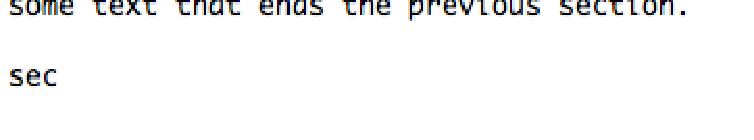
\includegraphics[width=.5\textwidth]{figs/startsec}}
\hfill\fbox{
\includegraphics[width=.5\textwidth]{figs/sec}}}
\makebox[\textwidth]{
\fbox{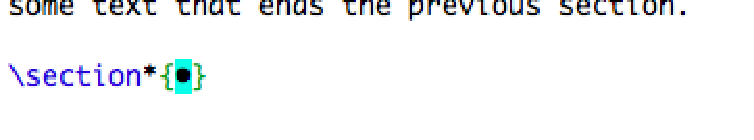
\includegraphics[width=.5\textwidth]{figs/secs}}
\hfill\fbox{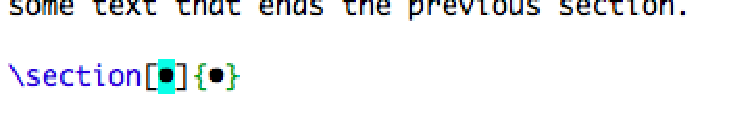
\includegraphics[width=.5\textwidth]{figs/seco}}}
\caption{De gauche à droite et de haut en bas cycle des résultats obtenus en entrant \texttt{sec} par pressions successives de \esckey\ : soit la séquence \textsf{initial}\To\textsf{sec}\To\textsf{secs}\To\textsf{seco}.}
\label{fig:sec}
\end{figure}

%\textbf{NOTE: The list may be a bit intimidating. There is no need to ``memorize'' all of these abbreviations; learn the minimum number as you need them. In addition variations on a given abbreviation are obtained by successive pressings of \esckey; e.g., see Figure \ref{fig:sec}.}
%\begin{figure}\centering
%\makebox[\textwidth]{
%\fbox{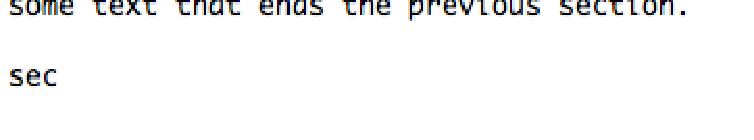
\includegraphics[width=3in]{figs/startsec}}
%\hfill\fbox{
\includegraphics[width=3in]{figs/sec}}}
%\makebox[\textwidth]{
%\fbox{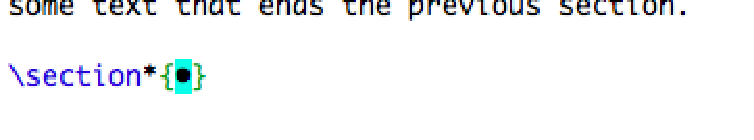
\includegraphics[width=3in]{figs/secs}}
%\hfill\fbox{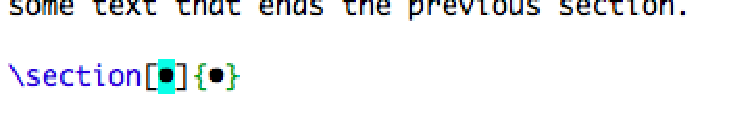
\includegraphics[width=3in]{figs/seco}}}
%\caption{Initially entered \texttt{sec} and successive pressings of \esckey\ from initial to last result before returning to the beginning. Corresponds to the sequence \textsf{initial}\To\textsf{sec}\To\textsf{secs}\To\textsf{seco}.}
%\label{fig:sec}
%\end{figure}

\subsection*{Abréviations des environnements}
%\subsection*{Environment Abbreviations}

Le \textsc{Tableau}~\Vref{tbl:environments} contient une liste des abréviations, pour différents environnements, 
fournies dans le fichier \CCT. Plusieurs environnements voisins verticalement portent le même nom. Ils correspondent à des variations dans le nombre et la répartition des arguments optionnels possibles ou à des variantes étoilées (\texttt{*}). Il se peut qu'il y ait, aussi, plus d'une abréviation pour le même environnement.

%Table (\ref{tbl:environments}) on page \pageref{tbl:environments} contains a list of abbreviations for different environments supplied in the \CCT\ file. Multiple vertically adjacent Environments with the same name correspond to variations in number and distribution of possible optional arguments or \texttt{*}-variants. There can also be more than one abbreviation for the same environment.

\subsection*{Commandes et déclarations}
%\subsection*{Commands \& Declarations}

Comme pour les environnements il y a beaucoup de variations, en options et variantes étoilées (\texttt{*}), ainsi que de nombreuses abréviations correspondant à la même commande : voir le \textsc{Tableau}~\Vref{tbl:commands}.

%As with Environments there are lots of variations with options and \texttt{*}-variants as well as multiple abbreviations corresponding to the same command. See Table (\ref{tbl:commands}) on page \pageref{tbl:commands}.

\subsection*{Lettres grecques}
%\subsection*{Greek Letters}

Les abréviations des lettres grecques apparaissent dans le \textsc{Tableau}~\Vref{tbl:greek}. Les versions destinées aux équations en ligne, c.-à-d., celles précédées d'un « \texttt{d} », ne sont pas présentées.

%The Greek Letter abbreviations appear in Table (\ref{tbl:greek}) on page \pageref{tbl:greek}. The in-line equation, i.e., `\texttt{d}', versions of the letters are not shown.

\section*{Ajouts au fichier \CCT}
%\section*{Making Additions to \CCT}

Si vous ajoutez des éléments au fichier \CCT{}, vous devez connaître certaines choses concernant sa structure :
%If you are adding items to the \CCT\ there are a few things you should know about its structure:
\begin{itemize}
\item Chaque environnement possède trois entrées : un complétement qui supprime le \verb|\begin| de tête, c.-à-d., qu'il commence avec une accolade « \texttt{\{} » et le nom de l'environnement ; deux abréviations qui ont un nom d'abréviation sans barre oblique inverse (\verb|\|) et l'abréviation, elle-même, avec la barre oblique inverse. Les commandes peuvent avoir plusieurs formes ; la commande intégrale ainsi qu'une ou plusieurs abréviations, toutes avec ou sans la barre oblique inverse \verb|\|.
\item Pour les abréviations, vous devez ajouter toutes les variantes de terminaisons légèrement différentes. J'utilise 
un « \texttt{o} », à la fin d'une abréviation, pour un argument optionnel ; un « \texttt{oo} » pour deux arguments facultatifs ; un « \texttt{s} » pour des commandes de formes étoilées, etc.
\item L'ordre d'éléments similaires, dans le fichier, amène \emph{vraiment} une différence importante dans l'ordre dans lequel ils sont trouvés : ceux placés \emph{après}, seront trouvés \emph{plus tôt} (l'exploitation du fichier est ascendante). Ainsi, l'ordre des éléments obtenus lorsque vous tapez \verb|\b| puis \esckey\ dépend purement de l'ordre des correspondances dans le fichier \CCT.
\item Pour un maximum de confort, placez un repère\footnote{En utilisant \mnu{Insérer un repère} (\cmdkey-\textsf{8}) du menu \mnu{Source}\To\mnu{Complètement}\To\mnu{Repères}.} dans chacun des arguments des commandes. Entourez le tout premier argument avec deux commandes \verb|#INS#| afin qu'il en ressorte sélectionné. Si vous voulez avoir un aide-mémoire dans tous les arguments, insérez la structure\footnote{En utilisant \mnu{Insérer un aide-mémoire} (\ctlkey-\cmdkey-\textsf{8}) du menu \mnu{Source}\To\mnu{Complètement}\To\mnu{Repères}.} nécessaire et remplissez-la.
\end{itemize}%\smallskip

Je suggère que vous jetiez un \oe{}il dans le fichier \CCT\ pour des exemples.

%\begin{itemize}
%\item
%Each environment has three entries: a completion that removes the leading \verb|\begin|, i.e., it starts with a leading `\texttt{\{}' and the environment name; two abbreviations that have an abbreviation name without a backslash (\verb|\|) and the same abbreviation with the backslash. Commands may have more forms; the full command as well as abbreviation(s) all with and without a leading \verb|\|.
%\item
%You should add all the variations with slightly different endings for the abbreviations. I use an `\texttt{o}' at the end of an abbreviation if that variation has an optional argument, `\texttt{oo}' for two optional arguments, `\texttt{s}' for \texttt{s}tarred forms of commands, etc.
%\item
%The order of similar items in the file \emph{does} make a dramatic difference in the order in which items are found; items placed \emph{later} will be found \emph{earlier} (the file is searched backwards). E.g., the order of items obtained when you press \verb|\b| and then \esckey\ depends purely on the order of matches in the \CCT\ file.
%\item
%For maximum convenience place a Mark\footnote{Using \mnu{Insert Mark} (\cmdkey-\textsf{8}) from the \mnu{Source}\To\mnu{Completion}\To\mnu{Marks} menu.} within each argument of commands. Surround the very first argument with two \verb|#INS#| commands so it comes out selected. If you want to have a comment in any arguments insert a Comment Skeleton\footnote{Using \mnu{Insert Comment} (\ctlkey-\cmdkey-\textsf{8}) from the \mnu{Source}\To\mnu{Completion}\To\mnu{Marks} menu.} and fill it in.
%\end{itemize}
%I'd suggest that you take a look in the \CCT\ file for examples.

\section*{Bogues}
%\section*{Bugs}

Le fichier \CCT\ est habituellement exploité de façon ascendante, à partir du dernier élément ; mais, dans de rares cas, le sens de la recherche semble s'inverser, si bien que vous n'obtenez pas les correspondances dans l'ordre que vous attendiez. Vous pouvez, généralement, forcer l'exploitation à revenir dans la « bonne » direction, en tapant \verb+---+ et en appuyant trois fois sur \esckey, et ensuite en enlevant le  \verb+---+. Si cela ne corrige pas le sens de la recherche, vous pouvez utiliser le raccourci \shiftkey\,-\,\esckey\ pour chercher dans l'« autre » direction.

%The \CCT\ file is usually searched backward from the last item but, on rare occasions, the search direction seems to switch so you don't get matches in the order you expect. You can usually force the search to go back to the ``correct'' direction by pressing \verb+---+ and then \esckey\ three times and then remove the \verb+---+. If that doesn't correct the direction you can use \shiftkey\,-\,\esckey\ to search in the ``other'' direction.

\section*{Ce qui manque}
%\section*{What's Missing}

Toutes les suggestions sont bienvenues et seront prises en considération afin d'être incluses dans les itérations 
ultérieures du code du complètement de commande. 

\vspace{5pt plus 2pt minus 1pt}\noindent
Essayez le… J'espère que vous l'aimerez.

%Any suggestions are welcome and will be considered for inclusion in later iterations of the Command Completion code.
%
%\vspace{5pt plus 2pt minus 1pt}\noindent
%Try it\dots\ I hope you like it.

%\vspace{5pt plus 2pt minus 1pt}\noindent
%Good Luck,\\
%Herb Schulz\\
%(\href{mailto:herbs2@mac.com}{herbs2@mac.com})

\begin{table}
\small
\centering
\caption{Abréviations des environnements dans \CCT.\label{tbl:environments}}
\begin{tabular}{llll}
\textbf{Abréviation} & \textbf{Environnement} & \textbf{Abréviation} & \textbf{Environnement} \\
%\begin{tabular}{llll}
%\textbf{Abbreviation} & \textbf{Environment} & \textbf{Abbreviation} & \textbf{Environment} \\
\cmidrule[0.5pt](lr){1-1} \cmidrule[0.5pt](lr){2-2} \cmidrule[0.5pt](lr){3-3} \cmidrule[0.5pt](lr){4-4}
barr      & array       & blett   & letter \\
babs      & abstract    & blist   & list \\
bali      & align       & bminp   & minipage \\
balis     & align*      & bminpo  & minipage \\
baliat    & alignat     & bmult   & multline \\
baliats   & alignat*    & bmults  & multline* \\
balied    & aligned     & bpict   & picture \\
baliedat  & alignedat   & bpmat   & pmatrix \\
baliedato & alignedat   & bquot   & quotation \\
bapp      & appendix    & bquo    & quote \\
bbmat     & bmatrix     & bsplit  & split \\
bcase     & cases       & bsubeq  & subequations \\
bcent     & center      & btab    & tabular \\
bcenum    & compactenum & btabs   & tabular* \\
bcenumo   & compactenum & btabx   & tabularx \\
bcitem    & compactitem & btabl   & table \\
bcitemo   & compactitem & btablo  & table \\
bdes      & description & btabls  & table* \\
benu      & enumerate   & btablso & table* \\
benuo     & enumerate   & btbl    & table \\
bequ      & equation    & btblo   & table \\
bequs     & equation*   & btbls   & table* \\
beqn      & eqnarray    & btblso  & table* \\
beqns     & eqnarray*   & btabb   & tabbing \\
bfig      & figure      & bbib    & thebibliography \\
bfigo     & figure      & bindex  & theindex \\
bframe    & frame       & btheo   & theorem \\
bframeo   & frame       & btitpg  & titlepage \\
bflalig   & flalign     & btrivl  & trivlist \\
bflaligs  & flalign*    & bvarw   & varwidth \\
bfll      & flushleft   & bverb   & verbatim \\
bflr      & flushright  & bvers   & verse \\
bgath     & gather      & bwrap   & wrapfigure \\
bgaths    & gather*     & bwrapo  & wrapfigure \\
bgathed   & gathered    & bwrapo2 & wrapfigure \\
bgathedo  & gathered    & bwrapoo & wrapfigure \\
bite      & itemize     &         & \\
biteo     & itemize     &         & \\
\end{tabular}
%\caption{Environment abbreviations supplied in \CCT.}
%\label{tbl:environments}
\end{table}

\begin{table}
\centering
\small
\caption{Commandes et déclarations dans \CCT.\label{tbl:commands}}
\makebox[\textwidth]{%
\begin{tabular}{llllll}
\textbf{Abréviation} & \textbf{Commande} & \textbf{Abréviation} & \textbf{Commande} & \textbf{Abréviation} & \textbf{Commande} \\
%\makebox[\textwidth]{%
%\begin{tabular}{llllll}
%\textbf{Abbreviation} & \textbf{Command} & \textbf{Abbreviation} & \textbf{Command} & \textbf{Abbreviation} & \textbf{Command} \\
\cmidrule[0.5pt](lr){1-1} \cmidrule[0.5pt](lr){2-2} \cmidrule[0.5pt](lr){3-3} \cmidrule[0.5pt](lr){4-4} \cmidrule[0.5pt](lr){5-5} \cmidrule[0.5pt](lr){6-6}
\texttt{-{}-}    & textendash        & midr       & midrule        & renewcomo       & renewcommand \\
\texttt{-{}-{}-} & textemdash        & mnorm      & mathnormal     & renewcomoo      & renewcommand \\
\texttt{-{}-{}-} & textemdash w/sp   & msf        & mathsf         & rncm            & renewcommand \\
adlen            & addtolength       & mtt        & mathtt         & rnewc           & renewcommand \\
adcount          & addtocounter      & mit        & mathit         & rncmo           & renewcommand \\
bf               & textbf            & midr       & midrule        & rnewcoo         & renewcommand \\
bfd              & bfseries          & mnorm      & mathnormal     & rncmoo          & renewcommand \\
biblio           & bibliography      & mdd        & mdseries       & rmc             & rmfamily \\
bibstyle         & bibliographystyle & mbox       & mbox           & rbox            & raisebox \\
botr             & bottomrule        & makebox    & makebox        & rboxo           & raisebox \\
bibitem          & bibitem           & mboxo      & makebox        & rboxoo          & raisebox \\
bibitemo         & bibitem           & makebox    & makebox        & sec             & section \\
center           & centering         & mboxoo     & makebox        & secs            & section* \\
chap             & chapter           & mpar       & marginpar      & seco            & section \\
cmidr            & cmidrule          & multic     & multicolumn    & ssec            & subsection \\
cmidro           & cmidrule          & ncol       & space \& space & ssecs           & subsection* \\
em               & emph              & ncm        & newcommand     & sseco           & subsection \\ 
emd              & em                & newc       & newcommand     & sssec           & subsubsection \\
foot             & footnote          & ncmo       & newcommand     & sssecs          & subsubsection* \\
frac             & frac              & newco      & newcommand     & ssseco          & subsubsection \\
fbox             & fbox              & ncmoo      & newcommand     & spar            & subparagraph \\
fboxo            & framebox          & newcoo     & newcommand     & spars           & subparagraph* \\
fboxoo           & framebox          & nct        & newcolumntype  & sparo           & subparagraph \\
geometry         & geometry          & newct      & newcolumntype  & setl            & setlength \\
hw               & headwidth         & newpg      & newpage        & stcount         & stepcounter \\
hw2tw            & headw\(=\)textw   & npg        & newpage        & sf              & textsf \\
href             & href              & nline      & newline        & sfd             & sffamily \\
item             & item              & newlin     & newline        & sc              & textsc \\
ito              & item              & nlen       & newlength      & scd             & scshape \\
incg             & includegraphics   & newlen     & newlength      & sl              & textsl \\
incgo            & includegraphics   & nenv       & newenvironment & sld             & slshape \\
it               & textit            & newenv     & newenvironment & sqrt            & sqrt \\
itd              & itshape           & nenvo      & newenvironment & sqrto           & sqrt \\
latex            & LaTeX             & newenvo    & newenvironment & tt              & texttt \\
latexs           & LaTeX w/sp        & nenvoo     & newenvironment & ttd             & ttfamily \\
latexe           & LaTeXe            & newenvoo   & newenvironment & tw              & textwidth \\
latexes          & LaTeXe w/sp       & pgref      & pageref        & tex             & TeX \\
label            & label             & par        & paragraph      & texs            & TeX w/sp \\
lbl              & label             & pars       & paragraph*     & tilde           & textasciitilde \\
lettrine         & lettrine          & paro       & paragraph      & topr            & toprule \\
lettrineo        & lettrine          & pgs        & pagestyle      & toc             & tableofcontents \\
listf            & listoffigures     & parbox     & parbox         & tableofcontents & tableofcontents \\
listt            & listoftables      & parboxo    & parbox         & tpgs            & thispagestyle \\
rule             & rule              & parboxoo   & parbox         & thispagestyle   & thispagestyle \\
ruleo            & rule              & parboxooo  & parbox         & up              & textup \\
mbf              & mathbf            & pbox       & parbox         & upd             & upshape \\
mrm              & mathrm            & pboxo      & parbox         & url             & url \\
mcal             & mathcal           & pboxoo     & parbox         & usep            & usepackage \\
msf              & mathsf            & pboxooo    & parbox         & usepo           & usepackage \\
mtt              & mathtt            & ref        & ref            & verb            & verb \\ 
mit              & mathit            & renewcom   & renewcommand   & verb2           & verb \\
\end{tabular}
}
%\caption{Commands and Declarations in \CCT.}
%\label{tbl:commands}
\end{table}

\begin{table}\small\centering
\caption{Lettres grecques dans \CCT\ (versions « \texttt{d} » non présentées).\label{tbl:greek}}
\begin{tabular}{llll}
\textbf{Abréviation} & \textbf{Commande} & \textbf{Abréviation} & \textbf{Commande} \\
%\begin{tabular}{llll}
%\textbf{Abbreviation} & \textbf{Command} & \textbf{Abbreviation} & \textbf{Command} \\
\cmidrule[0.5pt](lr){1-1} \cmidrule[0.5pt](lr){2-2} \cmidrule[0.5pt](lr){3-3} \cmidrule[0.5pt](lr){4-4}
xa  & alpha      & xph  & phi \\
xb  & beta       & xcph & Phi \\
xch & chi        & xvph & varphi \\
xd  & delta      & xps  & psi \\
xcd & Delta      & xcps & Psi \\
xe  & epsilon    & xs   & sigma \\
xve & varepsilon & xcs  & Sigma \\
xet & eta        & xvs  & varsigma \\
xg  & gamma      & xz   & zeta \\
xcg & Gamma      & xr   & rho \\
xio & iota       & xvr  & varrho \\
xl  & lambda     & xt   & tau \\
xcl & Lambda     & xth  & theta \\
xm  & mu         & xcth & Theta \\
xn  & nu         & xvth & vartheta \\
xo  & omega      & xu   & upsilon \\
xco & Omega      & xcu  & Upsilon \\
xp  & pi         & xx   & xi \\
xcp & Pi         & xcx  & Xi \\
xvp & varpi      &      & \\
\end{tabular}
%\caption{Greek Letters in \CCT. The `\texttt{d}' versions are not shown.}
%\label{tbl:greek}
\end{table}

\end{document}
